\documentclass[12pt]{article}
% Francais UTF8
\usepackage[french]{babel}
\usepackage[utf8]{inputenc}
\usepackage[T1]{fontenc}
\usepackage{lmodern}
\usepackage{graphicx}
\usepackage[small]{caption}
\usepackage{amsmath, amssymb}
\usepackage{fullpage}
\newcommand{\R}{\mathbb{R}}
\newcommand{\Z}{\mathbb{Z}}

\newcommand{\fig}[1]{\textsc{Figure}~\ref{#1}}
\newcommand{\eq}[1]{(\ref{#1})}

\newtheorem{theorem}{Théorème}
\newtheorem{definition}{Définition}

\begin{document}
\author{Gaspard Jankowiak \quad Antoine Levitt\\ Tuteur : Antoine Girard}
\title{Modèles de création d'opinion dans des réseaux sociaux}
\maketitle
\abstract{Bonjour}
\tableofcontents
\newpage


\section{Introduction}
Blabla


\section{Modèles de communautés}
\subsection{Définitions}
Dans toute la suite, $(V, E)$ désigne un graphe à $n$ n\oe uds et $m$
arêtes non orienté : les éléments de $E$ sont des ensembles à deux
éléments de $V$. Ce graphe représente un réseau de $n$ individus, liés
par des relations spécifiques au domaine d'intérêt. Par exemple, on
peut prendre pour $V$ les individus d'un réseau social en ligne (type
Facebook, Myspace ...), et pour $E$ leurs relations d'amitié : $\{i,
j\} \in E$ si et seulement si les individus $i$ et $j$ sont amis. À
chaque individu $i$ on associe une valeur réelle\footnote{Il est facile
de généraliser au cas multidimensionnel, mais on se restreindra ici à la
dimension 1.} $x_i$ représentant son opinion : l'état des opinions est
donc représenté par un vecteur $x \in \R^n$.

Tout d'abord, quelques rappels de théorie des graphes. On note $d_i$
le degré du n\oe ud $i$, égal au nombre d'arêtes incidentes au n\oe ud
$i$ : $d_i = card \{e \in E | i \in e\}$. À cette notion est
associée celle de {\bf matrice des degrés} $D$, matrice diagonale
de taille $n \times n$ telle que $D_{i i} = d_i$. On définit
également la {\bf matrice d'adjacence} $A$ telle que $A_{i j} = 1$
si $\{i, j\} \in E$, $0$ sinon. Le graphe étant non orienté, cette
matrice est symétrique.

On utilise ces notions pour construire la matrice qui nous sera
utile par la suite, la {\bf matrice Laplacienne}, définie par $L
= D - A$. On a donc $L_{i j} = d_i$ si $i = j$, $L_{i j} = 1$ si
$i$ est adjacent à $j$, et $L_{i j} = 0$ sinon. Son nom vient du
fait que c'est l'analogue pour un graphe quelconque de
l'opérateur Laplacien classique : pour un graphe représentant un
espace à $2$ dimensions discrétisé, c'est-à-dire dont les n\oe uds
sont les points $(i \Delta x, j \Delta y)$, on a $L(x) (i, j) =
4 x(i, j) - x(i+1, j) - x(i-1, j) - x(i, j+1) - x(i, j-1)$, et
on retrouve au signe près le Laplacien discrétisé. Les
propriétés (notamment spectrales) de cette matrice renseignent
sur le graphe, et c'est cette approche que l'on va utiliser dans
notre étude.

\subsection{Modélisation par équation différentielle}
Étant donné un vecteur d'opinions initiales $x(0)$, on
s'intéresse à l'évolution de ces opinions dans différents
modèles. Le modèle de base est l'équation différentielle
\begin{equation}
 \label{eq_diff}
 \dot x + L x = 0.
\end{equation}

On peut interpréter cette équation en la réécrivant composante par composante :
\begin{equation}
 \label{eq_diff_scal}
 \dot {x}_i = \sum_{j \in N_i} (x_j - x_i),
\end{equation}
où $N_i$ est le voisinage de $i$, c'est à dire tous les n\oe uds qui lui
sont adjacents. Chaque personne révise son opinion en fonction de
celle de ses voisins. Intuitivement, on s'attend à ce que ce modèle
provoque une convergence vers un consensus. Cette intuition est
corroborée par la ressemblance de (\ref{eq_diff}) avec l'équation de
la chaleur, dont les propriétés de convergence vers la valeur moyenne
sont bien connues. En fait, dans le cas d'un graphe représentant un
espace discrétisé, (\ref{eq_diff}) est tout simplement la
discrétisation par différences finies de l'équation de la chaleur. On
va maintenant démontrer ces propriétés de convergence.

\subsection{Propriétés spectrales de $L$}
\label{props_spectrales_L}
$L$ est symétrique donc diagonalisable dans une base orthonormée de
vecteurs propres $(v_i)_{i=1\dots n}$ associés à des valeurs propres
$(\lambda_i)_{i=1 \dots n}$. On décompose $x^0$ sur cette base : $x^0
= \sum_{i=1}^n \alpha_i v_i$, et la solution de (\ref{eq_diff}) ayant
cette condition initiale est $$x(t) = \sum_{i=1}^n \alpha_i e^{-
 \lambda_i t} v_i.$$ L'étude de la convergence de l'équation
différentielle passe donc par l'étude des valeurs propres de $L$.

La somme des lignes de $L$ est égale à $0$ (par définition du degré),
c'est-à-dire que $(1, 1, \dots, 1)^T$ est vecteur propre pour la valeur
$0$. On va montrer que $L$ est positive, c'est-à-dire que toutes ses
valeurs propres sont positives. Pour cela, on utilise la
caractérisation : une matrice est positive si et seulement si $x^T L x \geq 0$ pour
tout $x \in \R^n$.

\begin{eqnarray*}
 x^T L x & = & \sum_{i = 1}^n x_i \sum_{j \in N_i} (x_i - x_j) \\
 & = & \sum_{i = 1}^n d_i {x_i}^2 - \sum_{i = 1}^n \sum_{j \in N_i} x_i x_j \\
 & = & \sum_{\{i, j\} \in E} ({x_i}^2 + {x_j}^2) - 2 \sum_{\{i, j\} \in E} x_i x_j \\
 & = & \sum_{\{i, j\} \in E} (x_i - x_j)^2 \\
 & \geq & 0
\end{eqnarray*}

$L$ est donc positive. On voit également qu'un vecteur propre associé
à la valeur propre $0$ a la même valeur sur tous les n\oe uds d'une
composante connexe. La multiplicité de $0$ comme valeur propre est
donc égale au nombre de composantes connexes dans le graphe. On ne
considère ici que des graphes connexes, donc on peut ranger les
valeurs propres : $0 = \lambda_1 < \lambda_2 \leq \lambda_3 \leq \dots
\leq \lambda_n$. Le comportement en l'infini de (\ref{eq_diff}) est
donc trivial : il converge vers $(\alpha_1, \alpha_1, \dots,
\alpha_1)^T$ qui n'est autre que la valeur moyenne de $x^0$. La
vitesse de convergence est dictée par la deuxième valeur propre
$\lambda_2$ : $||x(t) - x_\infty|| \approx e^{-\lambda_2 t}$. Cette
valeur propre est appellée {\bf connectivité algébrique}, et mesure à
quel point un graphe est connecté. Notons aussi que $x(t) - x_\infty$
s'aligne sur le second vecteur propre $v_2$ : $x(t) - x_\infty \approx
\alpha_2 e^{-\lambda_2 t} v_2$. Cette remarque nous sera utile par la
suite.

\subsection{Modèle discret}
\label{mod_discret}
Plutôt que de simuler ce modèle directement, on va utiliser un modèle
discrétisé, qui a sensiblement les même propriétés tout en étant plus
facile à étudier. Ce modèle permet notamment de rajouter des effets
qui seraient plus délicats à manipuler, comme on le verra section
\ref{forçage}. L'idée la plus simple est d'utiliser la méthode d'Euler
sur (\ref{eq_diff}), qui donne la relation de récurrence en l'indice
discret $t$ :
\begin{equation}
 \label{eq_discrete}
 x(t+1) = x(t) - \alpha L x(t),
\end{equation}
ou sous forme scalaire :
\begin{equation}
 \label{eq_discrete_scal}
 x_i(t) = x_i(t) + \alpha \sum_{j \in N_i} (x_j(t) - x_i(t)).
\end{equation}

On retrouve l'idée de l'équation précédente : à chaque étape, chaque
individu modifie son opinion en fonction de celle de ses voisins. Le
paramètre $\alpha$ représente l'amplitude des changements par pas de
temps. Le modèle précédent est retrouvé dans la limite où $\alpha$
tend vers 0. Dans nos simulations, on prend $\alpha$ suffisamment
petit pour ne pas introduire d'oscillations parasites, et suffisamment
grand pour avoir des simulations rapides.

Notons que les valeurs propres de l'application itérée $I - \alpha L$
s'obtiennent à partir de celles de $L$ par la formule $\lambda = 1 -
\alpha \lambda_L$. Si $\alpha$ est suffisamment petit, tous ces
valeurs propres sont de valeur absolue strictement inférieure à $1$,
sauf une correspondant au vecteur propre $(1, 1, \dots, 1)^T$. En
triant les valeurs propres dans l'ordre $-1 < \lambda_n \leq
\lambda_{n-1} \leq \dots \leq \lambda_2 < \lambda_1 = 1$, on
retrouve bien la convergence vers la valeur moyenne à la vitesse
${\lambda_2}^t$, avec $\lambda_2 = 1 - \alpha \lambda_{L,2}$.

\subsection{Forçage et formation de communautés}
\label{forçage}
Les expériences numériques sur ce modèle donnent bien le résultat
attendu, c'est-à-dire un consensus, et la vitesse de convergence est
bien égale à la seconde valeur propre $\lambda_2$. On veut maintenant
utiliser ces résultats pour obtenir des résultats sur la structure du
graphe, et notamment l'existence de communautés dans celui-ci. L'idée
est simple : si on force les gens à se mettre d'accord plus vite
qu'ils ne se mettraient d'accord naturellement, il ne va pas y avoir
consensus mais formation de différents groupes de même
opinion. L'étude de ces groupes peut faire apparaître une structure de
communauté. Pour mettre en pratique ces idées, on impose à chaque
personne de ne prendre en considération que des avis raisonnablement
proche du sien, et de se fermer de plus en plus au cours du
temps. Cela conduit au même modèle que précédemment, hormis le fait que la
somme n'est plus prise sur le voisinage de la personne dans le graphe,
mais dans un sous-ensemble de celui-ci : $$N'_{i} = \{j \in N_i, ||x_i
- x_j|| < R \rho^t\}.$$

$R$ est un paramètre de normalisation, et $\rho$ caractérise la vitesse de
décroissance. Ce dernier paramètre est central dans notre étude. Pour
favoriser l'apparition de communautés de façon relativement indépendante des
conditions initiales, il faut que $R$ soit grand. En effet, dans le cas
contraire, des communautés se forment trop vite en fonction de la position
relative des données initiales.

Intuitivement, on s'attend à une bifurcation pour $\rho = \lambda_2$. En
effet, en supposant $R$ assez grand, le système va subir une phase transitoire
où les opinions vont s'homogénéiser, gommant la variabilités des conditions
initiales, puis converger vers l'équilibre à la vitesse ${\lambda_2}^t$. Si
$\lambda_2 < \rho$, la coupure n'interviendra pas, et le système convergera
vers un consensus tout comme dans le modèle précédent. Si $\lambda_2 > \rho$
en revanche, la convergence n'est pas assez rapide, et il y a coupure au bout
d'un certain temps : deux communautés s'isolent et fonctionnement
indépendamment l'une de l'autre. À partir de là, les deux communautés
convergent vers un consensus à des vitesses $\lambda_2^1$ et $\lambda_2^2$
(les connectivités algébriques des sous-graphes), et le même raisonnement
s'applique pour éventuellement diviser ces communautés davantage.

\section{Résultats}
Nous avons implémenté ce modèle en \textsc{MATLAB}, nous présentons ici
les principaux résultats.


\subsection{Graphes utilisés}
Nous allons nous intéresser à la formation de communautés. On ne peut
donc pas étudier des graphes aléatoires, et on utilise des graphes
existants, dont les communautés ont été observées expérimentalement.

Nous utilisons principalement deux graphes, représentés
\fig{exemples_graphes}. Le premier est le réseau d'amitié dans un club
de karaté d'une université américaine dans les années 70 contenant 34
membres, introduit par Zachary \cite{zachary}. Le second est le graphe
d'interactions d'une communauté de 62 dauphins \cite{dolphins}.

\begin{figure}[htb]
	\begin{center}
		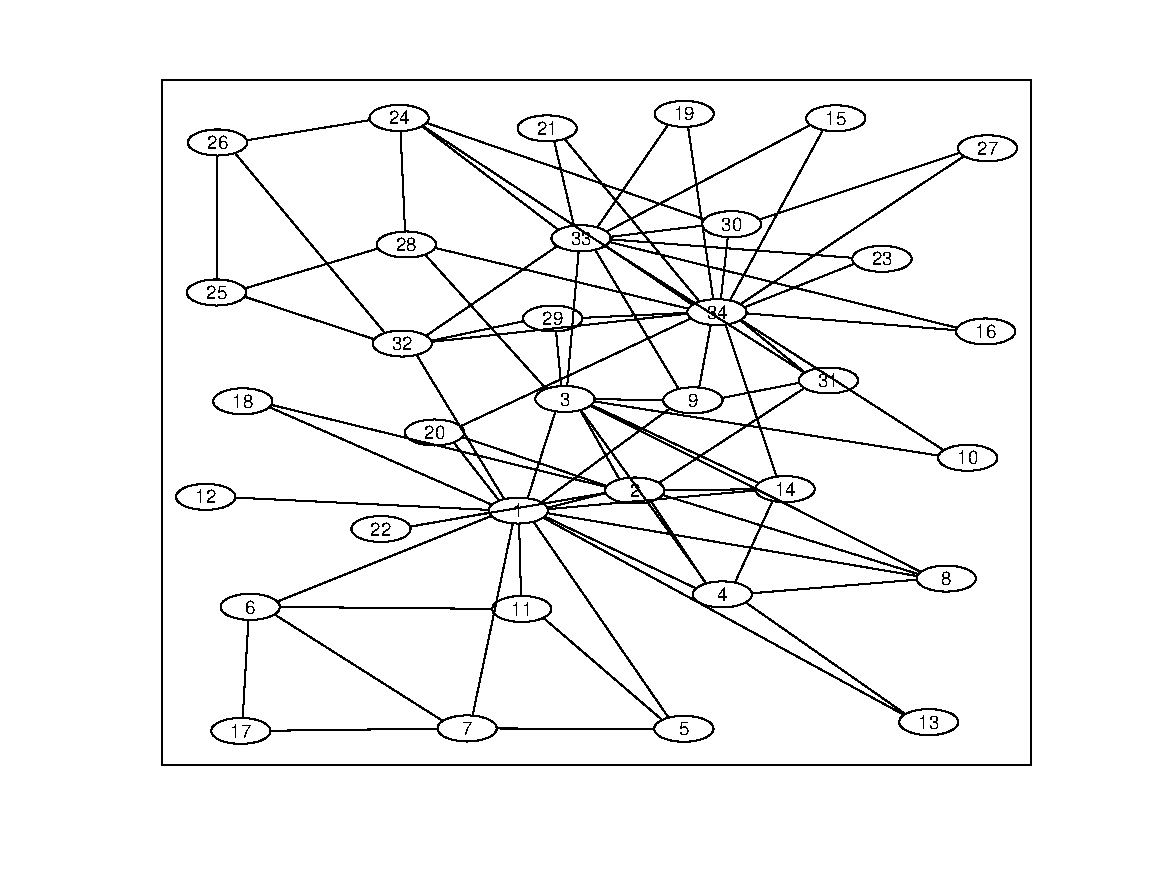
\includegraphics[width=.4 \textwidth]{zachary}
		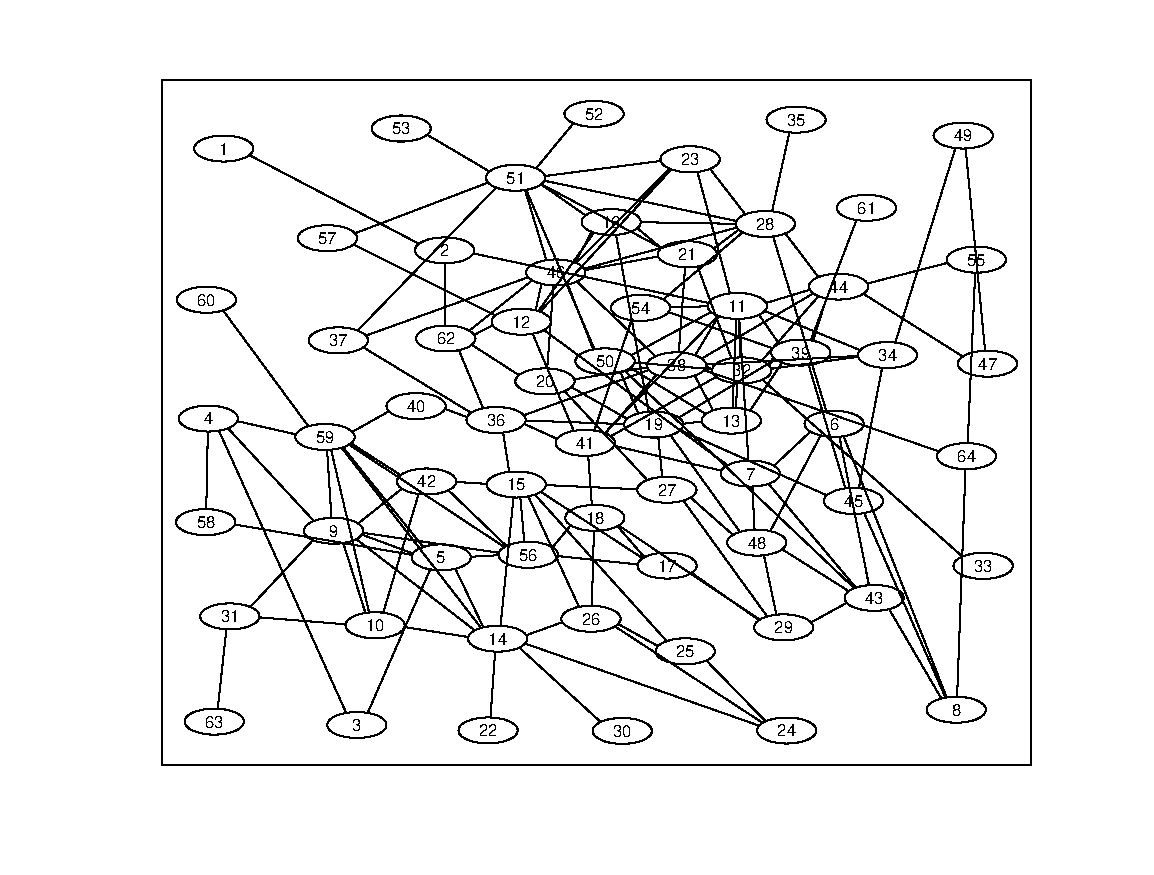
\includegraphics[width=0.4\textwidth]{dolphins}\\
		\hfill (a) \hfill (b) \hfill~\\
	\end{center}
	\caption{Club de karaté (a), et dauphins (b).}
	\label{exemples_graphes}
\end{figure}

Ces deux graphes sont intéressants parce qu'ils permettent de comparer
nos résultats à la réalité, des communautés ayant été mises en
évidence dans ces deux cas.

\subsection{Choix des paramètres}
Les opinions initiales sont tirés selon une loi uniforme sur $[0; 1]$.
$R$ est choisi relativement grand devant la taille de la distribution
initiale ($R\approx10$) pour éviter l'influence lors de la phase
transitoire, comme expliqué section \ref{forçage}. Enfin, $\alpha$ est
choisi de manière à avoir une simulation stable (voir section
\ref{mod_discret}) : en pratique, on prend $\alpha = 0,1$ pour le
graphe Zachary et $\alpha = 0,4$ pour les dauphins. On effectue $400$
itérations, ce qui produit des résultats peu sensibles aux conditions
initiales, et des simulations rapides.

\subsection{Détection des groupes}
Sans s'attacher à une définition formelle de la notion de communauté
(qui peut être complexe) on peut définir expérimentalement un
groupe. À l'instant $t$, on considère le graphe partiel $N'(t) =
\bigcup_i N'_i(t)$, c'est-à-dire la restriction du graphe original aux
agents qui communiquent encore. Ce graphe présente une ou plusieurs
composantes connexes, qui correspondent à autant de communautés
d'opinion.

\subsection{Évolution}

Voici l'évolution des opinions des différents agents, pour $\rho$
grand (première figure, une seule communauté) et $\rho$ petit (seconde
figure, formation de communautés à cause du forçage).

\begin{figure}[htb]
	\begin{center}
		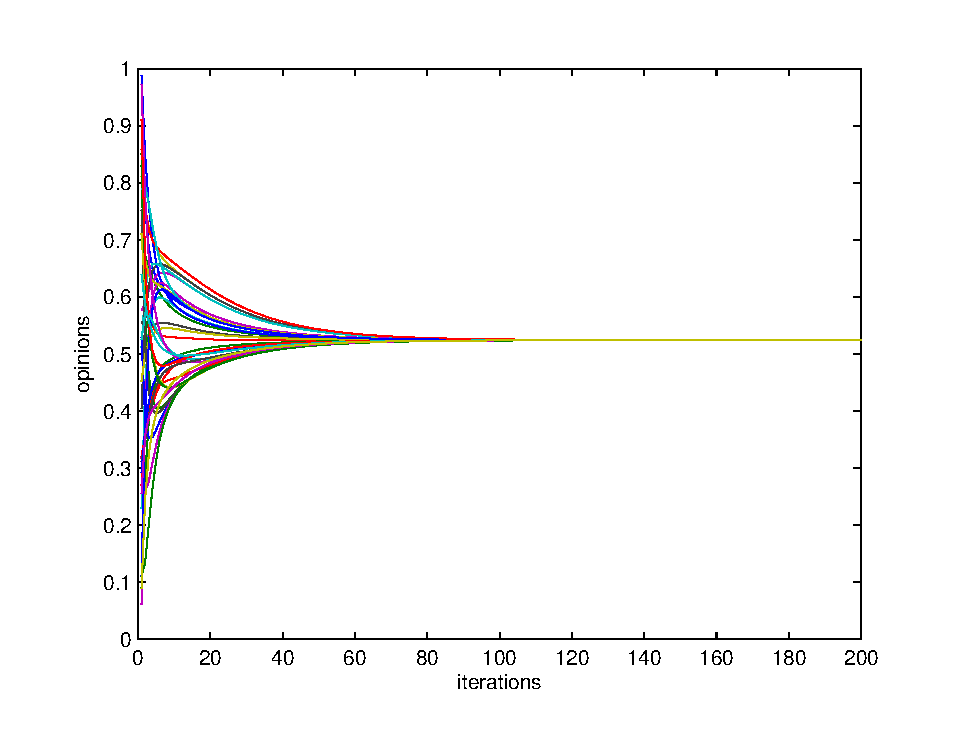
\includegraphics[width=.4\textwidth]{evolution_ok}
		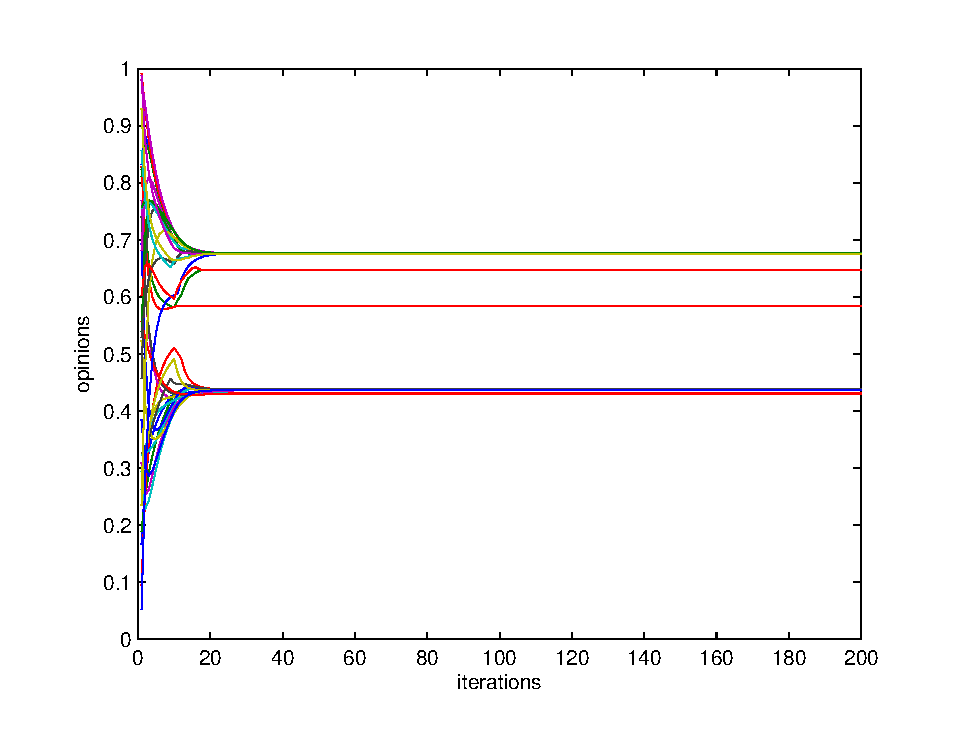
\includegraphics[width=.4\textwidth]{evolution_clusters}
	\end{center}
	\caption{Courbes d'évolution des opinions}
	\label{fig:evol}
\end{figure}

Nous voyons apparaître 2 phases (\fig{fig:evol}):
\begin{itemize}
	\item Une phase transitoire, où les opinions se rapprochent rapidement d'un <<~consensus~>>.
		Dans le cas de plusieurs groupes, plusieurs consensus se distinguent.
	\item Une phase de régime permanent : une fois les consensus atteints, aucune évolution n'est visible.
\end{itemize}


\subsection{Formation de communautés}
On visualise maintenant \fig{res_3cs} les résultats sur le graphe original, pour
$\rho < \lambda_2$. On observe des groupes au sein desquels l'opinion
est globalement homogène. Cette structure de groupe semble être peu
sensible à la répartition initiale des opinions et persiste
sur la plupart des simulations.

\begin{figure}[htb]
	\begin{center}
		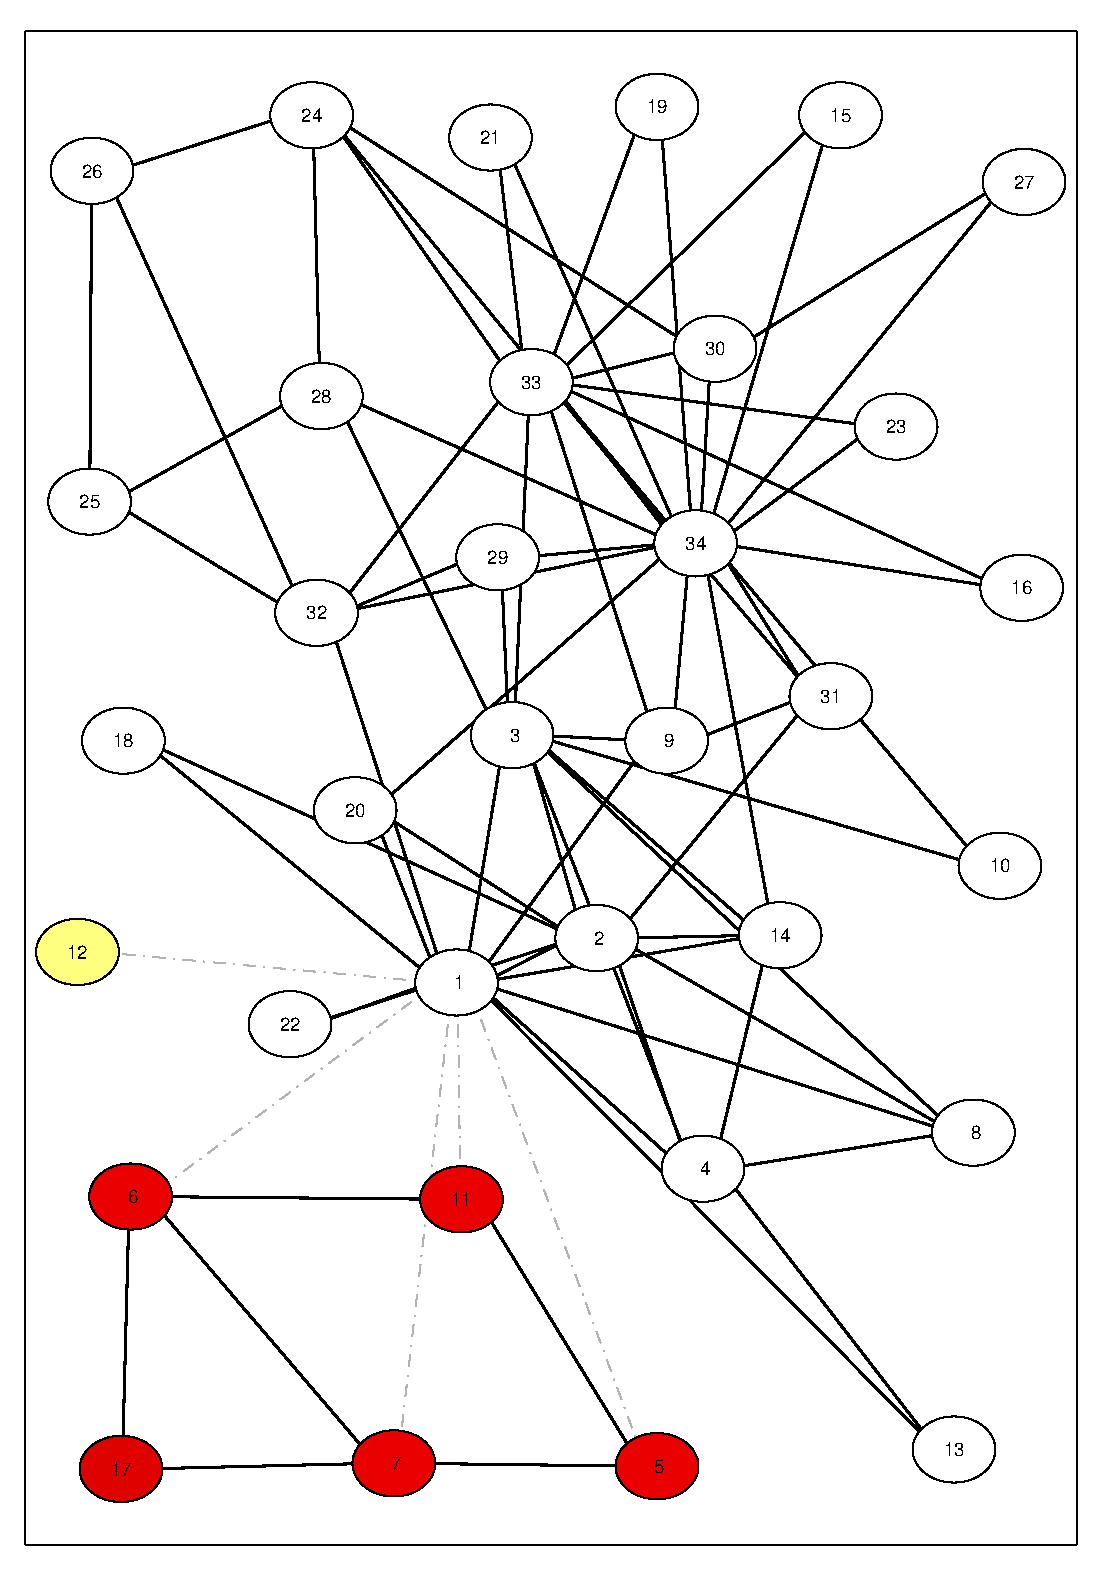
\includegraphics[width=.4\textwidth]{za-m1-3}
		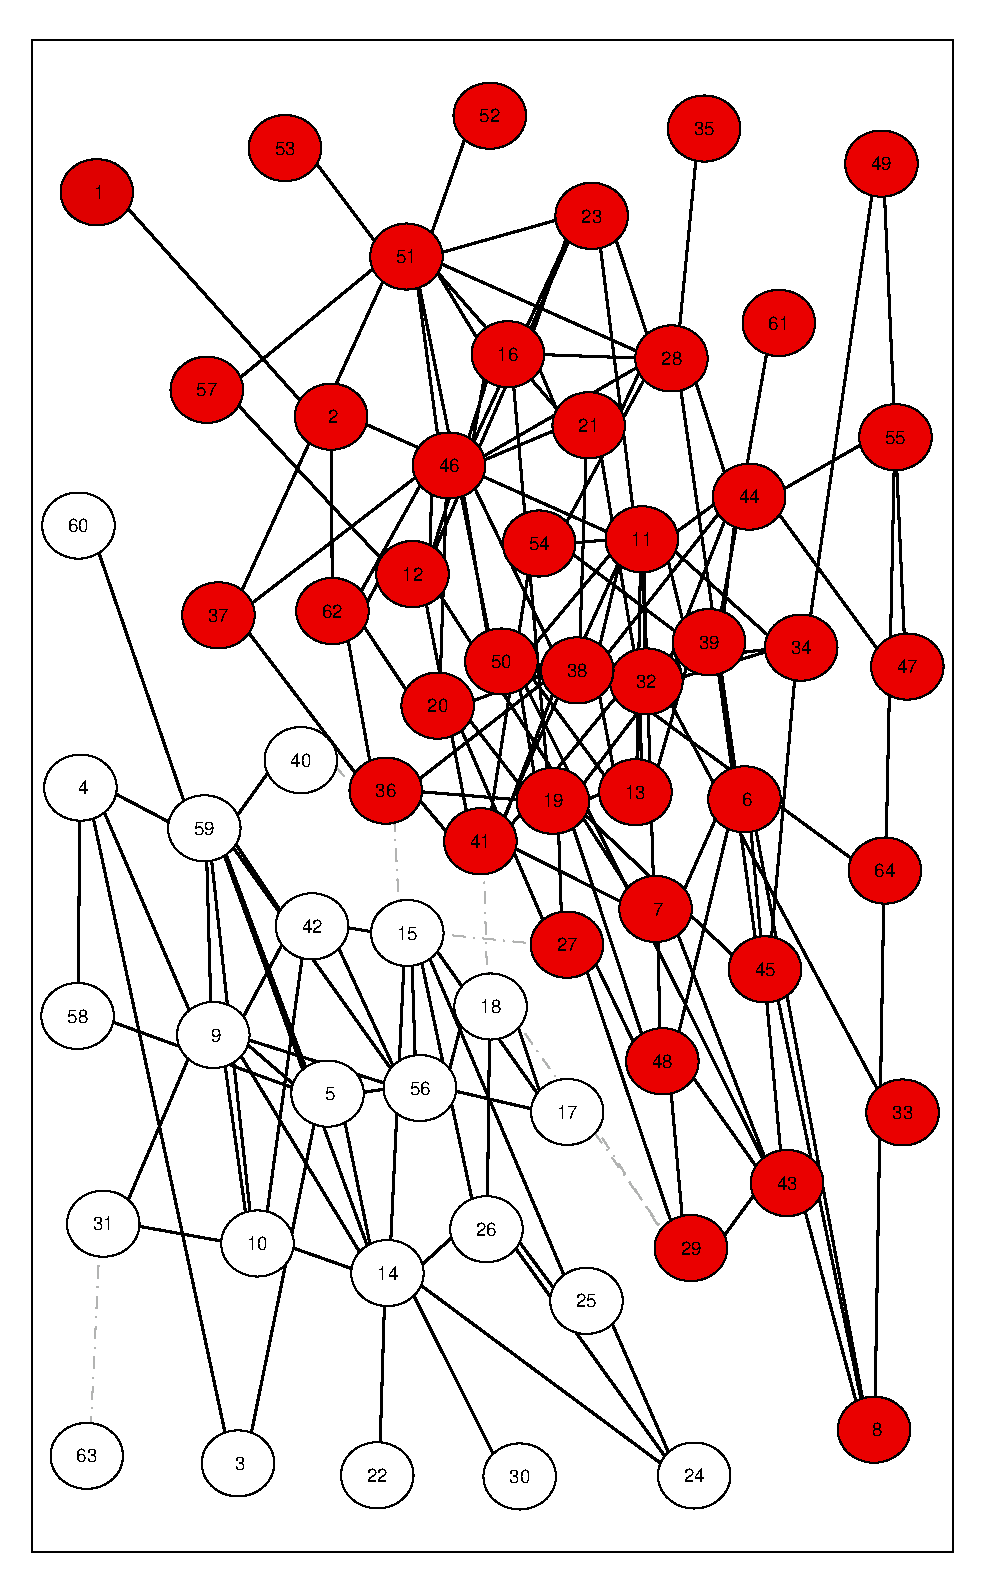
\includegraphics[width=.4\textwidth]{do-m1-3}
		\caption{Exemple de groupes apparaissant lors de la
 simulation. Les couleurs correspondent à l'opinion,
 et les liens détruits apparaissent en pointillés.}
		\label{res_3cs}
	\end{center}
\end{figure}

% Remarque : certains groupes sont relativement petits devant d'autre.

\subsection{Influence du forçage}
Figure et interprétation à changer

Maintenant nous nous intéressons à la bifurcation introduite en
section \ref{forçage}.  Pour ceci nous calculons le nombre de groupes
pour différentes valeurs de $\rho$ \fig{bifu_map}. $R$ est maintenu
suffisamment grand pour ne pas influer sur les résultats.  Nous
utilisons le graphe de Zachary, pour lequel $\lambda_2 \approx
0,953$.  Le nombre de groupe est calculé en faisant la moyenne sur 10
simulations.

\begin{figure}[htb]
	\begin{center}
		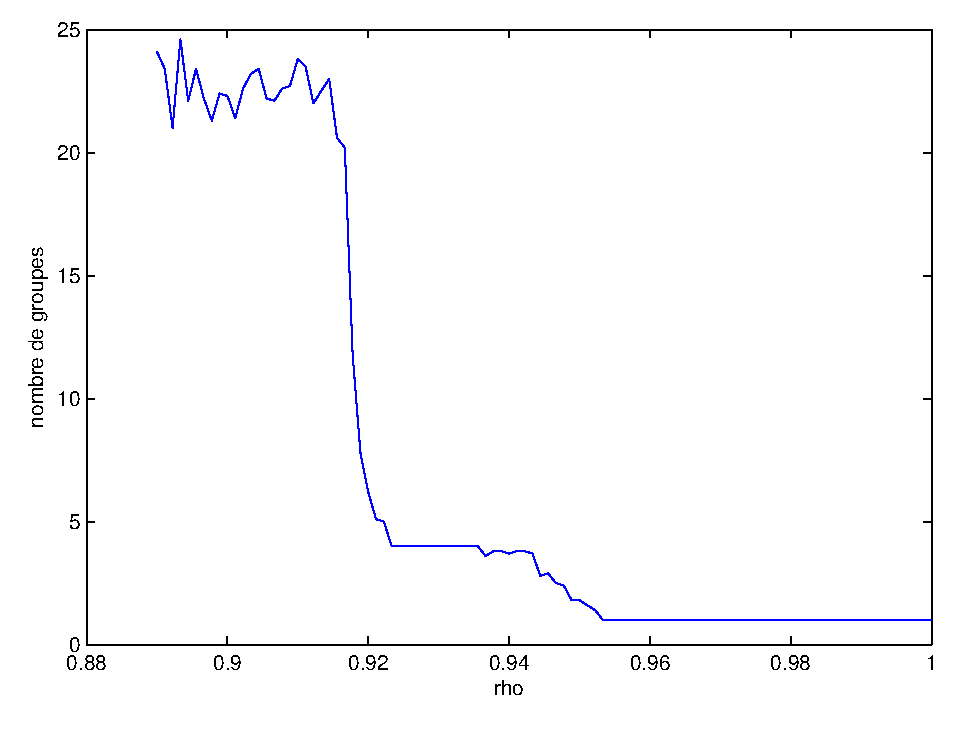
\includegraphics[width=0.5\textwidth]{bifur}
		\caption{Bifurcation pour $\rho < \lambda_2$}
		\label{bifu_map}
	\end{center}
\end{figure}

On observe bien un unique consensus pour $\rho$ suffisamment grand, et
de plus en plus de divisions quand on diminue $\rho$. On s'attend
à une bifurcation et à l'apparition de plusieurs communautés pour
$\rho = \lambda_2 = 0,953$. Cependant, l'apparition de divisions
n'apparaît que pour $\rho$ plus petit, vers $\lambda_2 = 0,94$.
\begin{figure}[htb]
	\begin{center}
		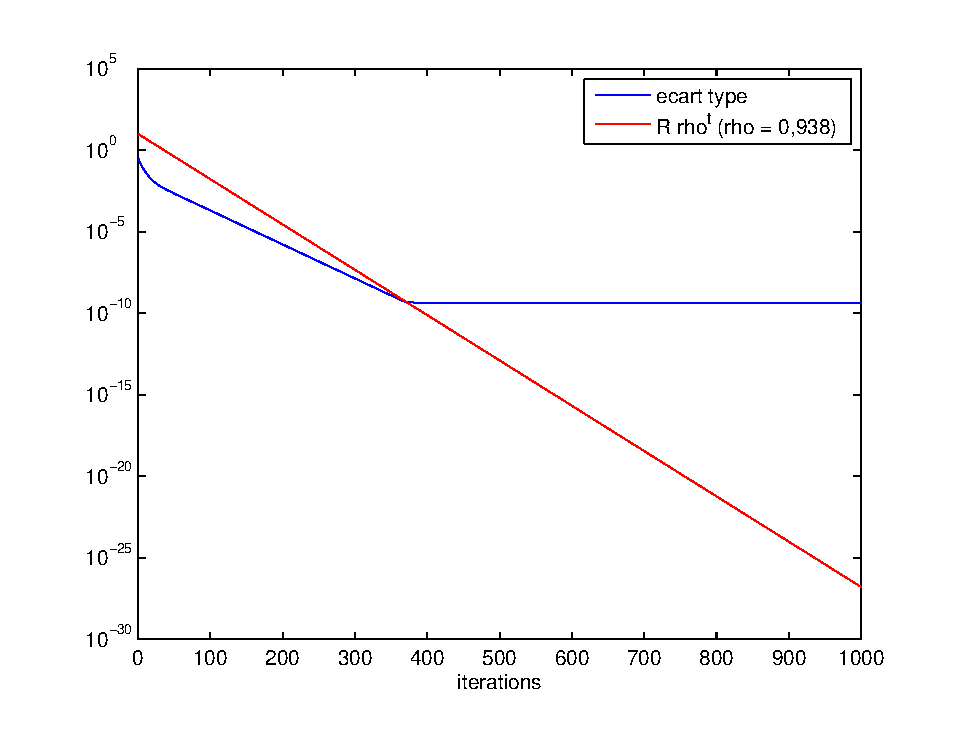
\includegraphics[width=.4\textwidth]{var_rho_0938}
		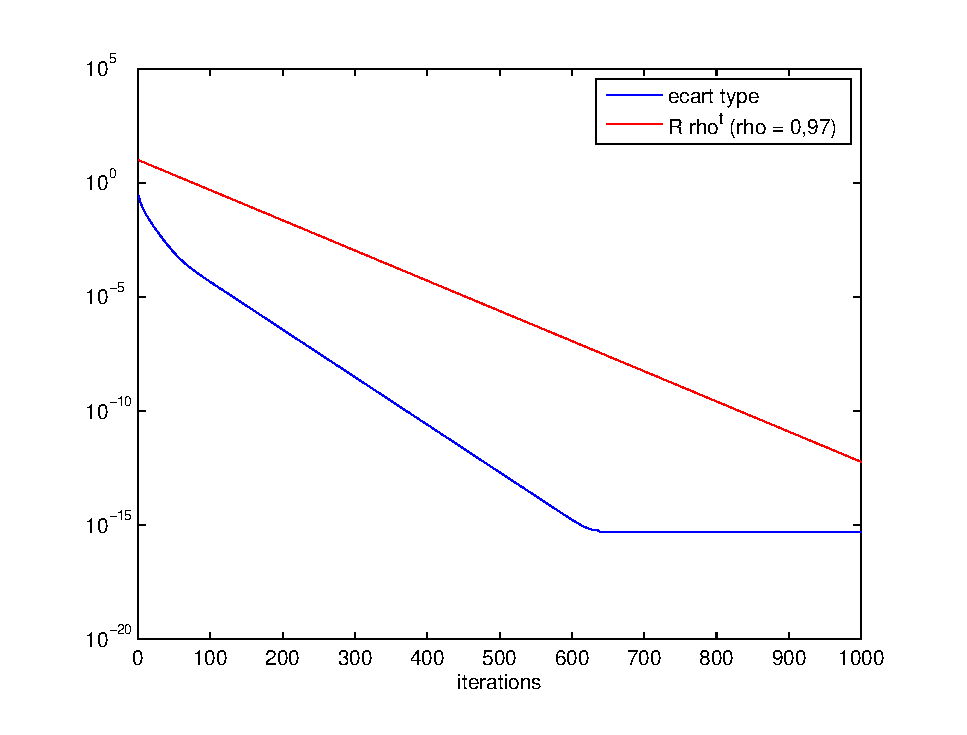
\includegraphics[width=.4\textwidth]{var_rho_097}
		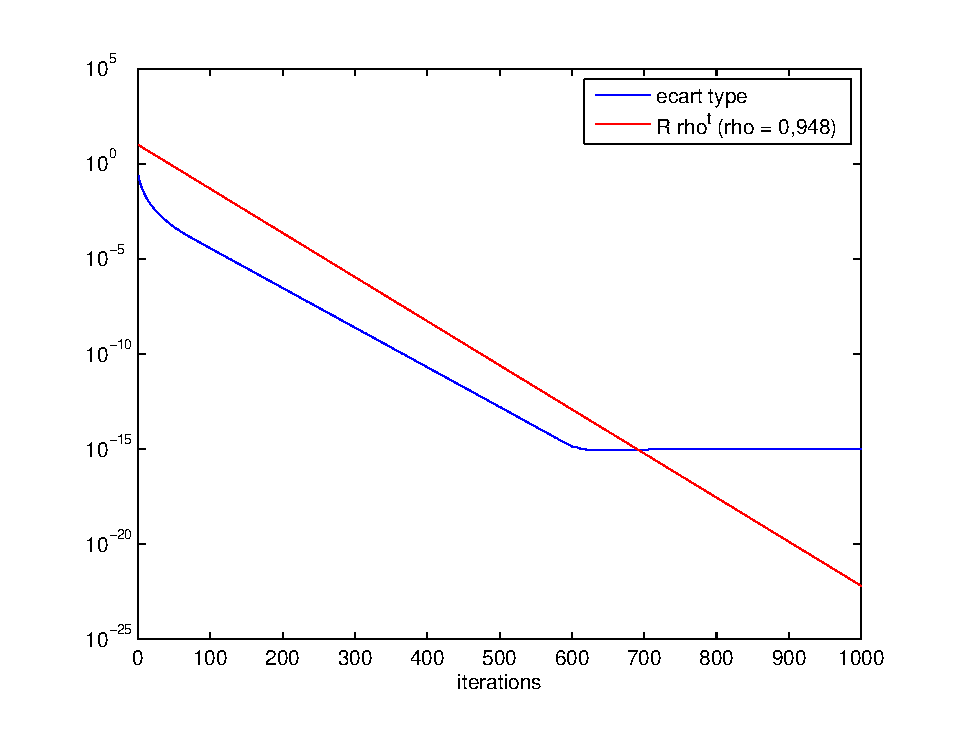
\includegraphics[width=.5\textwidth]{var_rho_0948}
		\caption{Évolution de l'écart type des opinions et
                  comparaison avec $R \rho^t$ pour $\rho = 0,938$,
                  $0,97$ et $0,948$. Échelle semi-logarithmique.}
		\label{num_coupure}
	\end{center}
\end{figure}
Ce phénomène est dû aux erreurs numériques. On représente
\fig{num_coupure} l'évolution de l'écart type (qui est égal à $||x -
x_\infty||$) en fonction du temps, et la courbe $R \rho^t$, pour
différentes valeurs de $\rho$.

\section{Partitionnement de graphes et détection de communautés}
Ces résultats montrent que le modèle fournit une méthode de
partitionnement d'un graphe. On va maintenant la comparer avec des
méthodes classiques de partitionnement.

\subsection{Partitionnement spectral}
Le problème à résoudre est : étant donné un graphe, comment le
partitionner de la façon la plus naturelle possible ? Évidemment, il
faut tout d'abord définir ce qu'on entend par <<~naturelle~>>. Un
critère qui peut être intéressant est le nombre d'arêtes entre les
deux groupes : on cherche la partition de $V$ en deux groupes $V_1$ et
$V_2$ qui minimise ce nombre d'arêtes $n_a$.

On note $x_p$ le vecteur caractérisant cette partition : il vaut 1 sur
$V_1$ et 0 sur $V_2$. Par le calcul mené au \ref{props_spectrales_L},
on a :

\begin{equation}
 x^T L x = \sum_{\{i, j\} \in E} (x_i - x_j)^2.
\end{equation}

Appliqué à notre vecteur $x$, on obtient
\begin{equation}
 x_p^T L x_p = n_a
\end{equation}

Ainsi notre problème s'écrit : trouver $x \in \{0,1\}^n$ qui
minimise $x^T L x$. C'est un problème d'optimisation combinatoire
qui peut être coûteux à résoudre quand $n$ est grand, et une
énumération triviale mène à une complexité en $\mathcal O (2^n)$. On peut
cependant en obtenir une approximation par une méthode spectrale. On
considère le problème analogue en domaine continu : $x$ est
maintenant pris dans la sphère unité de $R^n$. $L$ est symétrique donc
diagonalisable en base orthonormée à valeurs propres réelles, et on
peut écrire :

\begin{equation}
 x^T L x = \sum_{i=1}^n \lambda_i {x_i}^2,
\end{equation}
où $x_i$ est la composante de $x$ sur le vecteur propre $v_i$.

La solution à ce problème de minimisation est simple : mettre tout le
poids dans la somme sur la plus petite valeur propre, c'est-à-dire, en
supposant que les valeurs propres sont triées, prendre $x$ parallèle à
$v_1$. Comme vu précédemment, $\lambda_1 = 0$ et $v_1 = (1, 1, \dots,
1)^T$, ce qui donne une solution triviale du problème. Cette solution
consiste à mettre tous les n\oe uds dans $V_1$ : $n_a = 0$, mais ce
n'est pas très intéressant. On fixe donc la composante sur $v_1$ à 0,
et la solution est maintenant de prendre $x$ parallèle à $v_2$.

Il faut maintenant remonter au problème original discret, en
discrétisant la solution trouvée $v_2$. Par exemple, on peut vouloir
chercher le vecteur $x$ de $\{0,1\}^n$ qui maximise le parallélisme
$(x|v_2)$ avec $v_2$, ce qui conduit à mettre les entrées positives de
$v_2$ dans $V_1$ et les négatives dans $V_2$, ou le contraire. On peut
également grouper les composantes de $v_2$ pour chercher les deux
parties les mieux isolées, ce qui conduit à couper $v_2$ au point où
la différence $v_2(i) - v_2(i-1)$ est la plus grande.

Cette solution donne de bons résultats approchés pour le problème de
minimisation. Un avantage est qu'il existe des algorithmes efficaces
pour calculer $v_2$ (basés sur la méthode des
puissances). Typiquement, pour un graphe non pathologique (nombre
d'arêtes de l'ordre du nombre de n\oe uds), l'algorithme de
partitionnement est en $\mathcal O(n^2)$.

\subsection{Liens avec notre modèle}
On va maintenant expliciter les liens existant entre notre modèle
d'évolution d'opinion et la méthode de partitionnement spectral. Tout
d'abord, remarquons que notre méthode consiste à itérer l'application
$B = I - \alpha L$. Cette application possède les mêmes vecteurs
propres que $L$, et ses valeurs propres s'obtiennent par la
transformation affine $\lambda_B = 1 - \alpha \lambda_L$. À l'infini,
on a $x(t) - x_\infty \approx \alpha_2 {\lambda_2}^t v_2$, où
$\lambda_2$ est la seconde plus grande valeur propre de $B$ et $v_2$
le vecteur propre associé, qui est également le vecteur propre associé
à la seconde plus petite valeur propre de $L$.

En supposant $R$ assez grand, après un transitoire, $x(t)$ satisfait
l'approximation ci-dessus et est aligné sur $v_2$. La coupure dûe au
terme $R \rho^t$ intervient après le transitoire, et on s'attend à ce
que les opinions soient séparées en deux groupes en fonction du plus
grand écart de $v_2$ : on retrouve bien le partitionnement spectral.

\subsection{Laplacienne normalisée}
L'inconvénient de cette méthode est qu'elle cherche uniquement à
minimiser le nombre d'arcs entre les groupes. Elle risque donc
d'isoler de très petits groupements. Pour pallier à ce défaut, on
utilise donc BLABLA renormalisé.

\subsection{Résultats}

\section{Conclusion}
bonsoir

\clearpage
\begin{thebibliography}{2}
\bibitem{zachary} W. W. Zachary, An information flow model for conflict and fission in small groups, Journal of Anthropological Research 33, 452-473 (1977)
\bibitem{dolphins} D. Lusseau, K. Schneider, O. J. Boisseau, P. Haase, E. Slooten, and S. M. Dawson, Behavioral Ecology and Sociobiology 54, 396-405 (2003)
\end{thebibliography}
\end{document}
